%-------------------------------------
% Barcode Verification Report Template
%-------------------------------------

%---- Required Packages and Functions ----

\documentclass[a4paper,11pt]{report}
\usepackage{latexsym}
\usepackage{xcolor}
\usepackage{float}
\usepackage{ragged2e}
\usepackage[empty]{fullpage}
\usepackage{wrapfig}
\usepackage{lipsum}
\usepackage{tabularx}
\usepackage{titlesec}
\usepackage{geometry}
\usepackage{marvosym}
\usepackage{verbatim}
\usepackage{enumitem}
\usepackage[hidelinks]{hyperref}
\usepackage{fancyhdr}
\usepackage{multicol}
\usepackage{graphicx}
\usepackage{cfr-lm}
\usepackage[T1]{fontenc}
\setlength{\multicolsep}{0pt}
\pagestyle{fancy}
\fancyhf{}
\fancyfoot{}
\renewcommand{\headrulewidth}{0pt}
\renewcommand{\footrulewidth}{0pt}
\setlength{\footskip}{4.08003pt} % Fix for the footskip warning}
\geometry{left=1.4cm, top=0.8cm, right=1.2cm, bottom=1cm}
% Adjust margins
%\addtolength{\oddsidemargin}{-0.5in}
%\addtolength{\evensidemargin}{-0.5in}
%\addtolength{\textwidth}{1in}
\usepackage[most]{tcolorbox}
\tcbset{
	frame code={}
	center title,
	left=0pt,
	right=0pt,
	top=0pt,
	bottom=0pt,
	colback=gray!20,
	colframe=white,
	width=\dimexpr\textwidth\relax,
	enlarge left by=-2mm,
	boxsep=4pt,
	arc=0pt,outer arc=0pt,
}

\urlstyle{same}

\raggedright
\setlength{\tabcolsep}{0in}

% Sections formatting
\titleformat{\section}{
  \vspace{-4pt}\scshape\raggedright\large
}{}{0em}{}[\color{black}\titlerule \vspace{-7pt}]


% \renewcommand{\labelitemii}{$\circ$}
\renewcommand{\labelitemi}{$\vcenter{\hbox{\tiny$\bullet$}}$}

\newcolumntype{L}{>{\raggedright\arraybackslash}X}%
\newcolumntype{R}{>{\raggedleft\arraybackslash}X}%
\newcolumntype{C}{>{\centering\arraybackslash}X}%
%---- End of Packages and Functions ------

%-------------------------------------------
%%%%%% DEFINE ELEMENTS HERE %%%%%%%
\newcommand{\addressa}{Address line 1}
\newcommand{\addressb}{Address line 2}
\newcommand{\addressc}{Address line 3}
\newcommand{\phone}{XXXXXXXXX}
\newcommand{\email}{something@example.com}
\newcommand{\website}{https://gitlab.com/bashrc2/datamatrix}
\newcommand{\issuedate}{2025-07-20}
\newcommand{\symboltype}{Datamatrix}
\newcommand{\matrixsize}{NxN}
\newcommand{\overallgrade}{A}
\newcommand{\decoderesult}{ABCDEF}
\newcommand{\isosymbolgrade}{4.0 PASS}
\newcommand{\symbolcontrast}{A}
\newcommand{\modulation}{A}
\newcommand{\axialnonuniformity}{A}
\newcommand{\gridnonuniformity}{A}
\newcommand{\unusederrorcorrection}{A}
\newcommand{\fixedpatterndamage}{A}
\newcommand{\clocktrackregularity}{A}
\newcommand{\minreflectance}{A}
\newcommand{\lightaperture}{x.x}
\newcommand{\lightnm}{670}
\newcommand{\lightangle}{90}
\newcommand{\angleofdistortion}{0.1}
\newcommand{\contrastuniformity}{0}
\newcommand{\dotsperelement}{310}
\newcommand{\elongation}{22.7}
\newcommand{\quietzone}{100}
\newcommand{\distributeddamage}{0}
\newcommand{\cellfill}{40}

\begin{document}
\fontfamily{cmr}\selectfont
%----------HEADING-----------------
\parbox{2.8cm}{%

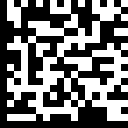
\includegraphics[width=2.5cm,clip]{img/logo_square.png}
% replace the fields with your details

}\parbox{\dimexpr\linewidth-3.1cm\relax}{
\begin{tabularx}{\linewidth}{L r}
  \textbf{\LARGE Barcode Verification} & Tel: \phone\\
  \addressa &  \href{mailto:\email}{\email}\\
  \addressb &  \href{\website}{Website}\\
  \addressc &  {\issuedate}
    \end{tabularx}
}


% %-----------METRICS-----------------
\section{Testing Summary}
\setlength{\tabcolsep}{5pt} % Default value: 6pt
\small{\begin{tabularx}
    {\dimexpr\textwidth-3mm\relax}{|c|C|}
    \hline
    \textbf{GS1 Parameters } & \textbf{Values}\\
\hline
Illumination  & \lightaperture/\lightangle/\lightnm\\
\hline
ISO symbol grade  & \isosymbolgrade\\
\hline
Symbol type  & \symboltype\\
\hline
Decode  & \decoderesult\\
\hline
Matrix size  & \matrixsize\\
\hline
\end{tabularx}}
\vspace{2mm}

% %-----------IMAGE-----------------
\begin{center}
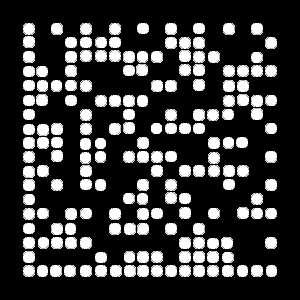
\includegraphics[width=11.0cm,clip]{img/datamatrix.png}
\end{center}

% %-----------GRADED METRICS-----------------
\section{Graded Metrics}
\setlength{\tabcolsep}{5pt} % Default value: 6pt
\small{\begin{tabularx}
    {\dimexpr\textwidth-3mm\relax}{|c|C|}
    \hline
    \textbf{ISO/IEC Parameters } & \textbf{Grade A-F}\\
    \hline
    Overall ISO Grade & \overallgrade \\
    \hline
    Symbol Contrast & \symbolcontrast \\
    \hline
    Modulation & \modulation \\
    \hline
    Axial non-uniformity & \axialnonuniformity \\
    \hline
    Grid non-uniformity & \gridnonuniformity \\
    \hline
    Unused Error Correction (UEC) & \unusederrorcorrection \\
    \hline
    Fixed pattern damage & \fixedpatterndamage \\
    \hline
    Clock track regularity & \clocktrackregularity \\
    \hline
    Minimum reflectance & \minreflectance \\
    \hline
\end{tabularx}}
\vspace{-2mm}

% %-----------NON-GRADED METRICS-----------------
\section{Non-Graded Metrics}
\setlength{\tabcolsep}{5pt} % Default value: 6pt
\small{\begin{tabularx}
    {\dimexpr\textwidth-3mm\relax}{|c|C|}
    \hline
    \textbf{Parameters } & \textbf{Values}\\
    \hline
    Angle of distortion (degrees) & \angleofdistortion \\
    \hline
    Contrast uniformity & \contrastuniformity \\
    \hline
    Dots per element & \dotsperelement \\
    \hline
    Elongation \% & \elongation \\
    \hline
    Quiet zone \% & \quietzone \\
    \hline
    Distributed damage \% & \distributeddamage \\
    \hline
    Cell fill \% & \cellfill \\
    \hline
\end{tabularx}}
\vspace{-2mm}

%-------------------------------------------
\end{document}
